%%%%%%%%%%%%%%%%%%%%%%%%%%%%%%%%%%%%%%%%%%%%%%%%%%%%%%%%%%%%%%%%%%%%%%%%%%%%%%%%
%
% \chapter{Post-process}\label{chPostProcess}
%
%%%%%%%%%%%%%%%%%%%%%%%%%%%%%%%%%%%%%%%%%%%%%%%%%%%%%%%%%%%%%%%%%%%%%%%%%%%%%%%%

This chapter provides a detailed explanation of all the output files generated by ERMES 20.0 after completing a computation. It also demonstrates how to use the GiD post-processor to visualize and analyse the results.

\section{Output files}

Several output files are generated by ERMES 20.0 upon completing the calculations. These output files can be categorized into the following groups:
\begin{itemize}\itemsep0em 
	\item Progress file,
	\item Visualization files,
	\item Surface integrals files,
	\item Volume integrals files,
	\item Scattering parameters files,
	\item Fields on nodes files.
\end{itemize}
In the following subsections, each group of output files will be detailed, including examples and format specifications. These files can be utilized to review the results, process them further using scripts, and conduct analyses. The results can be visualized using the GiD post-processor or, if preferred, with any other post-processing tool after reformatting them to be compatible with the chosen software.

\subsection{Progress file}\label{ssInfoFile}

The progress of an ERMES 20.0 computation is logged in the \path{Problem_Name.info} file located within the problem folder, where \path{Problem_Name} corresponds to the name of the problem currently being executed. This file can be opened directly with any text editor or 
viewed within the GiD pre-processor by clicking on \textbf{\underline{C}alculate} $\rightarrow$ \textbf{View process info...} in the GiD upper menu.

The \path{Problem_Name.info} file contains details about the problem's main settings, the residual error evolution of the solvers, and, upon completion of the calculation, the results of surface and volume integrals, as well as the scattering parameters, if any of these outputs were selected as described in Section \ref{FieldIntegrals}. An example of a \path{Problem_Name.info} file is shown below:
\begin{small}\begin{lstlisting}
ERMES analysis started...

Problem  type: Full wave
Geometry type: 3D
Element  type: RME 1st
AV potentials: Off
Stabilization: On
Angular  freq: 1e+09 Hz
[...]
------------------------------------------------------------
[...]
|S11| = -1.772862e-01 dB [ 9.797961e-01, -7.970637e-01 rad ]
|S21| = -1.409555e+01 dB [ 1.973433e-01, -2.818825e+00 rad ]
------------------------------------------------------------
[...]
------------------------------------------------------------
Volume[1]: 1.75e-07 m^3
[...]
VolIntg( Ey ) = 6.608089e-04 * exp( j * -3.046219e+00 )
VolIntg( Ez ) = 1.883837e-07 * exp( j * -7.014302e-01 )
[...]
VolIntg( (JxB)x ) = +3.768553e-06 + j * +4.910668e-01
VolIntg( (JxB)y ) = +6.360195e-09 + j * -2.813885e+00
[...]
------------------------------------------------------------
[...]
------------------------------------------------------------
Surface[3]: 5e-05 m^2
[...]
SrfIntg( Bx ) = 2.000487e-09 * exp( j * +3.482370e-01 )
SrfIntg( By ) = 4.660085e-11 * exp( j * -2.664756e+00 )
[...]
SrfIntg( |E| ) = 1.721156e+00
SrfIntg( |H| ) = 7.823491e-02
[...]
------------------------------------------------------------
[...]
Printing vector iE...
Printing vector rE...
Printing double mod(E)...
Printing vector iH...
[...]

ERMES analysis finished.
\end{lstlisting}\end{small} 
The surface integral results \ref{ssSurfaceIntSel} are denoted as \path{SrfIntg(.)}, and the surface is identified as \path{Surface[sId]}, where \path{sId} represents the unique identification number of the surface. Similarly, the volume integral results \ref{ssVolIntSel} are denoted as \path{VolIntg(.)}, and the volume is identify as \path{Volume[vId]}, where \path{vId} represents the unique identification number of the volume. The scattering parameters \ref{ssScatteringParaSel} are presented in decibels as \path{Sji(dB) = 20*log10(|Sji|)} and in polar form as \path{[|Sji|, phase(Sji) rad]}.

\subsection{Visualization files}\label{ssVisualizationFiles}

By default, ERMES 20.0 saves the simulation results in a binary file named \path{Problem_Name.flavia.res}, where \path{Problem_Name} corresponds to the name of the problem being solved. This file is located in the problem folder and can be read directly by the GiD post-processor. Section \ref{GiDPostProcess} provides instructions on how to visualize and analyse this file with the GiD post-processor. The file is generated with the help of the \path{gidpost} library, located in the source code folder \path{\ERMES_CPP_20.0\external_libraries\gidpost}. Additional details about this library are available in the GiD documentation.

If the \textit{Ascii} option is selected in the \textit{Output format} setting of \ref{ImportExportSettings}-\ref{Win-PSettings-3}, two files will be generated: \path{Problem_Name.post.res} and \path{Problem_Name.post.msh}. The first file contains the results, while the second provides information about the mesh. These files are human-readable and can be easily processed by other applications. However, they are slower to load in the GiD post-processor and consume more disk space compared to the binary format. An example of the mesh file \path{Problem_Name.post.msh} is provided below:
\begin{small}\begin{lstlisting}
MESH "HOMesh" dimension 3 ElemType Tetrahedra Nnode 4
Coordinates
1 0 0.01 0
2 0 0.01 0.0005
3 0 0.00926775 0
4 0.000760075 0.01 0
[...]
1249 0.045 0.000741483 0.0005
1250 0.045 0 0
1251 0.045 0 0.0005
End Coordinates
Elements
1 36 23 32 22 1
2 73 53 54 59 1
3 97 89 92 75 1
4 73 70 77 75 1
[...]
3396 582 619 616 610 2
3397 598 616 595 579 2
3398 562 600 572 561 2
End Elements
\end{lstlisting}\end{small} 
The file lists first the coordinates of each node in the mesh, followed by the connectivity of these nodes in the tetrahedral mesh, along with the material identification number assigned to each element. For the results file \path{Problem_Name.post.res}, an example is provided below:
\begin{small}\begin{lstlisting}
GiD Post Results File 1.0
GaussPoints "GPsEM_01" ElemType Tetrahedra
Number Of Gauss Points: 1
Natural Coordinates: Internal
End GaussPoints
GaussPoints "GPsEM_04" ElemType Tetrahedra
Number Of Gauss Points: 4
Natural Coordinates: Internal
End GaussPoints
Result "iE" "ERMES" 0 Vector OnNodes
Values
1 -354.667 368.144 0
2 -430.484 446.843 0
3 0.188047 0 0
[...]
1250 -0.00123668 0.0012949 0
1251 -0.0010276 0.00107598 0
End Values
Result "rE" "ERMES" 0 Vector OnNodes
Values
1 16.7959 -17.4341 0
2 23.6727 -24.5723 0
[..]
1250 0.0121584 -0.0127307 0
1251 0.00950394 -0.00995131 0
End Values
Result "mod(E)" "ERMES" 0 Scalar OnNodes
Values
1 511.766
2 621.409
[...]
1250 0.0176947
1251 0.0138408
End Values
[...]
Result "E(t)" "ERMES" 1.03125e-09 Vector OnNodes
Values
1 -52.7189 54.7222 0
2 -60.7654 63.0745 0
[...]
1250 0.0116835 -0.0122335 0
1251 0.00912084 -0.00955018 0
End Values
\end{lstlisting}\end{small} 
In the example above, results are presented for each node in the mesh. Alternatively, results can be provided at Gauss points by selecting either the \textit{GP 1} or \textit{GP 4} options in the \textit{Results mode} setting, as described in \ref{GeneralSettings}-\ref{Win-PSettings-1}. For further details about these files and their format, refer to the GiD documentation.

\subsection{Surface integrals files}\label{ssSurfaceIntFiles}

When the \textit{Field surface integral} option in \ref{Win-Integral-Surfs} is assigned to a surface, the integrals described in \ref{ssSurfaceIntSel} are automatically computed and saved in a file named \path{Surface-sId-Integrals.dat}, where \path{sId} represents the surface's identification number. This file is stored in the \path{\Integrals} folder within the problem directory. The format of \path{Surface-sId-Integrals.dat} is as follows:
\begin{small}\begin{lstlisting}
# Header
Freq |siEx| phsiEx |siEy| phsiEy |siEz| phsiEz si(|E| ) si(|E|^2)
Freq |siHx| phsiHx |siHy| phsiHy |siHz| phsiHz si(|H| ) si(|H|^2)
Freq |siBx| phsiBx |siBy| phsiBy |siBz| phsiBz si(|B| ) si(|B|^2)
Freq |siJx| phsiJx |siJy| phsiJy |siJz| phsiJz si(|J| ) si(|J|^2)
Freq |siSx| phsiSx |siSy| phsiSy |siSz| phsiSz si(|Jn|) si(r(Sn))
\end{lstlisting}\end{small} 
where \path{# Header} refers to a block of comments at the beginning of the file, outlining the file format and specifying the identification number of the surface. Each line in the header starts with the symbol \path{#}. Following the header, the results of the integrals are saved in polar form. \path{Freq} represents the frequency at which the integrals are calculated. \path{Freq} can be $f$ or $s$ depending on the frequency mode selected in \ref{Win-PSettings-4}-\ref{ProblemFreqSettings}. \path{si} denotes a complex surface integral, being \path{|si|} the magnitude of the complex integral and \path{phsi} its phase. \path{S} refers to a magnitude twice the time average of the Poynting vector \path{S} = $2\left\langle\mathbf{S}\right\rangle = \mathbf{E}_{c}\times\mathbf{\bar{H}}_{c}$. \path{|Jn|} is the magnitude of the normal component of the current density at the surface, and \path{r(Sn)} represents the real part of the normal component of \path{S}. If the \emph{Sweep frequency mode} option in \ref{ProblemFreqSettings}-\ref{Win-PSettings-4} is selected, this block will be repeated for each frequency within the interval specified in \ref{Win-PSettings-4}.

\subsection{Volume integrals files}\label{ssVolumeIntFiles}

When the \textit{Field volume integral} option in \ref{Win-Integral-Vols} is assigned to a volume, the integrals described in \ref{ssVolIntSel} are automatically computed and saved in a file named \path{Volume-vId-Integrals.dat}, where \path{vId} represents the volume's identification number. This file is stored in the \path{\Integrals} folder within the problem directory. The format of \path{Volume-vId-Integrals.dat} is as follows:
\begin{small}\begin{lstlisting}
# Header
Freq |viEx| phviEx |viEy| phviEy |viEz| phviEz vi(|E|) vi( |E|^2 )
Freq |viHx| phviHx |viHy| phviHy |viHz| phviHz vi(|H|) vi( |H|^2 )
Freq |viBx| phviBx |viBy| phviBy |viBz| phviBz vi(|B|) vi( |B|^2 )
Freq |viJx| phviJx |viJy| phviJy |viJz| phviJz vi(|J|) vi( |J|^2 )
Freq |viFx| phviFx |viFy| phviFy |viFz| phviFz vi(|F|) vi(r(J*.E))
\end{lstlisting}\end{small} 
where \path{# Header} refers to a block of comments at the beginning of the file, outlining the file format and specifying the identification number of the volume. Each line in the header starts with the symbol \path{#}. Following the header, the results of the integrals are saved in polar form. \path{Freq} represents the frequency at which the integrals are calculated. \path{Freq} can be $f$ or $s$ depending on the frequency mode selected in \ref{Win-PSettings-4}-\ref{ProblemFreqSettings}. \path{vi} denotes a complex volume integral, being \path{|vi|} the magnitude of the complex integral and \path{phvi} its phase. \path{F} represents the cross product $\mathbf{J}_{c}\times\mathbf{B}_{c}$, and \path{r(J*.E)} = $Real[\,\mathbf{\bar{J}}_{c}\cdot\mathbf{E}_{c}\,]$. If the \emph{Sweep frequency mode} option in \ref{ProblemFreqSettings}-\ref{Win-PSettings-4} is selected, this block will be repeated for each frequency within the interval specified in \ref{Win-PSettings-4}.

\subsection{Scattering parameters files}\label{ssScatteringParaFiles}

When the \textit{Projection RWTE10} or \textit{Projection CoaxialTEM} options in \ref{Win-Integral-Surfs} are assigned to a waveguide port surface, the scattering parameters \ref{ssScatteringParaSel} are automatically calculated and saved in a file named \path{SParameter-S_j_i.dat}, where \path{j} and \path{i} denote the identification numbers of the ports. This files is stored in the \path{\Integrals} folder within the problem directory. The format of the \path{SParameter-S_j_i.dat} file is as follows:
\begin{small}\begin{lstlisting}
# Header
Freq   Sji(dB)   |Sji|   phSji
\end{lstlisting}\end{small} 
where \path{# Header} refers to a block of comments at the beginning of the file, outlining the file format and specifying the identification number of the waveguide port. Each line in the header begins with the symbol \path{#}. Following the header, the scattering parameters are provided in decibels and polar form. In this case, unlike the surface and volume integral files, \path{Freq} represents only the frequency $f$ at which the scattering parameters are calculated, noting that complex frequencies $s$ are not available for waveguide port boundary conditions. \path{Sji(dB)} = $20\log_{10}{(\,|Sji|\,)}$, \path{|Sji|} is the module of the scattering parameter $S_{ji}$, and \path{phSji} its phase. If the \emph{Sweep frequency mode} option in \ref{ProblemFreqSettings}-\ref{Win-PSettings-4} is selected, this line will be repeated for each frequency within the specified interval.

\subsection{Fields on nodes files}\label{ssFieldsOnNodesFiles}

If the \emph{Export fields} option in \ref{ImportExportSettings}-\ref{Win-PSettings-3} is set to \textit{On}, and there are surfaces or volumes with the \textit{Field surface integral} or \textit{Field volume integral} options assigned to them, the fields $\mathbf{E}_{c}$, $\mathbf{B}_{c}$, $\mathbf{H}_{c}$, and $\mathbf{J}_{c}$ for those surfaces or volumes will be saved to files in the \path{\Fields} folder, located within the problem folder. If there are the surfaces assigned, the fields will be saved to files named:
\begin{itemize}\itemsep0em 
	\item \path{Surface_sId_E.dat},
	\item \path{Surface_sId_B.dat},
	\item \path{Surface_sId_H.dat},
	\item \path{Surface_sId_J.dat},
\end{itemize}
where \path{sId} represents identification number of the surface. If there are the volumes assigned, the fields will be saved to files named:
\begin{itemize}\itemsep0em 
	\item \path{Volume_vId_E.dat},
	\item \path{Volume_vId_B.dat},
	\item \path{Volume_vId_H.dat},
	\item \path{Volume_vId_J.dat},
\end{itemize}
where \path{vId} represents the identification number of the volume. Moreover, a set of files containing information about the nodes and elements of the mesh of the selected surfaces and volumes will also be saved alongside the field files in the \path{\Fields} folder. The names of the files detailing the mesh information are listed below:
\begin{itemize}\itemsep0em 
	\item \path{Surface_sId_Nodes.dat},
	\item \path{Surface_sId_Elements.dat},
	\item \path{Volume_vId_Nodes.dat},
	\item \path{Volume_vId_Elements.dat}.
\end{itemize}
The format of the files \path{Surface_sId_Nodes.dat} and \path{Volume_vId_Nodes.dat} is the following:
\begin{small}\begin{lstlisting}
# Freq(Hz)
NodeId  X(m)  Y(m)  Z(m)
\end{lstlisting}\end{small} 
where \path{Freq(Hz)} is the problem frequency in $Hz$, which can be $f$ or $s$ depending on the frequency mode selected (see \ref{Win-PSettings-4}-\ref{ProblemFreqSettings}), \path{NodeId} is the identification number of a node on the selected surface or volume, and \path{X(m)}, \path{Y(m)}, and \path{Z(m)} are the Cartesian coordinates of the node in $m$. The format of the file \path{Surface_sId_Elements.dat} is:
\begin{small}\begin{lstlisting}
# Freq(Hz)
NodeId_1  NodeId_2  NodeId_3
\end{lstlisting}\end{small} 
where \path{NodeId_1}, \path{NodeId_2}, and \path{NodeId_3} represent the identification numbers of the nodes of a triangular element on the selected surface. A similar format is used for the selected volumes in the files named \path{Volume_vId_Elements.dat}:
\begin{small}\begin{lstlisting}
# Freq(Hz)
NodeId_1  NodeId_2  NodeId_3  NodeId_4
\end{lstlisting}\end{small} 
where \path{NodeId_1}, \path{NodeId_2}, \path{NodeId_3}, and \path{NodeId_4} represent the identification numbers of the nodes of a tetrahedral element on the selected volume. The complex electric field $\mathbf{E}_{c}$ on the selected surfaces and volumes will be stored in the files \path{Surface_sId_E.dat} and \path{Volume_vId_E.dat} with the format:
\begin{small}\begin{lstlisting}
# Freq(Hz)
Real(Ecx)  Imag(Ecx)  Real(Ecy)  Imag(Ecy)  Real(Ecz)  Imag(Ecz)
\end{lstlisting}\end{small} 
where \path{Ecx}, \path{Ecy}, and \path{Ecz} are the Cartesian components of the complex electric field $\mathbf{E}_{c}$ in $V/m$. The complex magnetic flux density $\mathbf{B}_{c}$ on the selected surfaces and volumes will be stored in the files \path{Surface_sId_B.dat} and \path{Volume_vId_B.dat} with the format:
\begin{small}\begin{lstlisting}
# Freq(Hz)
Real(Bcx)  Imag(Bcx)  Real(Bcy)  Imag(Bcy)  Real(Bcz)  Imag(Bcz)
\end{lstlisting}\end{small} 
where \path{Bcx}, \path{Bcy}, and \path{Bcz} are the Cartesian components of the complex magnetic flux density $\mathbf{B}_{c}$ in $T$. The complex magnetic field $\mathbf{H}_{c}$ on the selected surfaces and volumes will be stored in the files \path{Surface_sId_H.dat} and \path{Volume_vId_H.dat} with the format:
\begin{small}\begin{lstlisting}
# Freq(Hz)
Real(Hcx)  Imag(Hcx)  Real(Hcy)  Imag(Hcy)  Real(Hcz)  Imag(Hcz)
\end{lstlisting}\end{small} 
where \path{Hcx}, \path{Hcy}, and \path{Hcz} are the Cartesian components of the complex magnetic field $\mathbf{H}_{c}$ in $A/m$. The complex electric current density $\mathbf{J}_{c}$ on the selected surfaces and volumes will be stored in the files \path{Surface_sId_J.dat} and \path{Volume_vId_J.dat} with the format:
\begin{small}\begin{lstlisting}
# Freq(Hz)
Real(Jcx)  Imag(Jcx)  Real(Jcy)  Imag(Jcy)  Real(Jcz)  Imag(Jcz)
\end{lstlisting}\end{small} 
where \path{Jcx}, \path{Jcy}, and \path{Jcz} are the Cartesian components of the complex electric current density $\mathbf{J}_{c}$ in $A/m^{2}$. The order of the field files aligns with the nodes file, such that the first line of a field file corresponds to the value of the field at the first node in the nodes file, and so on. If the \emph{Sweep frequency mode} is selected, the fields for each frequency will be stored in their corresponding files, with each frequency block separated by the line: \path{# Freq(Hz)}. 

\section{GiD postprocess}\label{GiDPostProcess}

The GiD post-processor can be accessed from the GiD pre-processor upper menu by selecting \textbf{\underline{F}iles} $\rightarrow$ \textbf{Postprocess} or by clicking the rainbow icon located in the upper-right corner of the GiD pre-processor. To return to the GiD pre-processor from the GiD post-processor, select \textbf{\underline{F}iles} $\rightarrow$ \textbf{Preprocess} or click on the corresponding icon in the upper-right corner of the GiD post-processor. If the problem has been loaded in pre-process, switching to post-process will automatically open the corresponding results file. However, if the post-processor is opened empty, the results files \path{.flavia.res} or \path{.post.res} must be manually loaded from \textbf{\underline{F}iles} $\rightarrow$ \textbf{Open}.

Once the results are loaded in the post-processor, it may be necessary to frame the geometry by clicking on \textbf{\underline{V}iew} $\rightarrow$ \textbf{Zoom} $\rightarrow$ \textbf{Frame}. After framing, open the \textit{View Results} window \ref{PostResults-Win} from the upper menu \textbf{\underline{W}indow} $\rightarrow$ \textbf{View results...}. In the \textit{View Results} window, choose a \textbf{View} (e.g., \textit{Contour Fill}, \textit{Display Vectors}, etc.) and then select a magnitude to visualize. Complex magnitudes are stored in \textbf{Step}: \textbf{0.0}, whereas time-domain values are stored in the subsequent time steps.

\begin{figure}[H]
	\begin{center}
		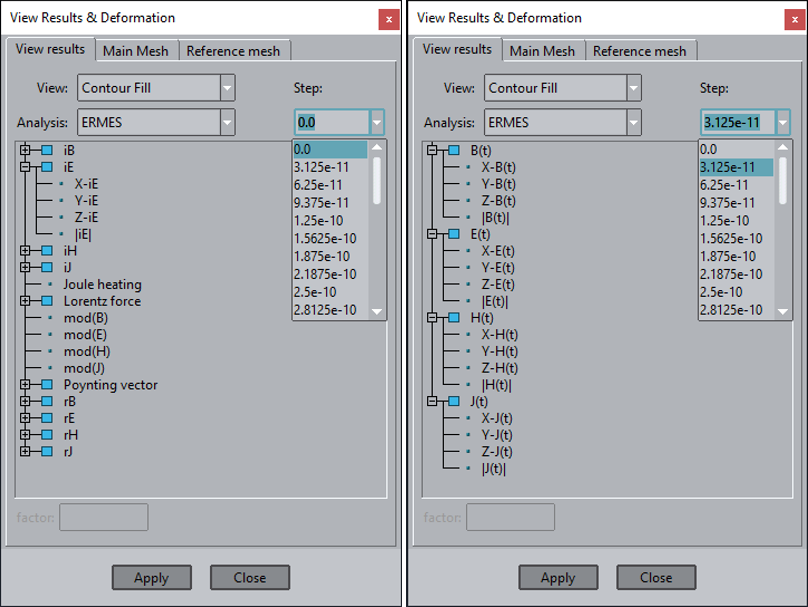
\includegraphics[width=0.80\textwidth]{Contents/Figures/PostResults-Win.png}
		\caption{\textit{View Results} window displaying the available results for two different time steps.}\label{PostResults-Win}
	\end{center}
\end{figure}

\noindent The upper menu \textbf{\underline{W}indow} provides access to various result-related windows, such as:
\begin{itemize}\itemsep0em 
	\item \textbf{View results...}: selects results to visualize (see Figure \ref{PostResults-Win}).
	\item \textbf{Animate...}: animates time-domain results and records videos. 
	\item \textbf{View graphs...}: displays and creates customized graphs.
	\item \textbf{View style...}: selects layers and adjust rendering styles.
\end{itemize}
The upper menu \textbf{V\underline{i}ew results} provides access to various result visualization styles and operations, including: \textbf{Contour fill}, \textbf{Contour lines}, \textbf{Show min max}, \textbf{Display vectors}, \textbf{Iso surfaces}, \textbf{Stream lines}, \textbf{Graphs}, \textbf{Results surface}, and \textbf{Integrate}.

Visualization settings can be adjusted through the \textit{Preferences Window}. This window is accessible via the upper menu \textbf{\underline{U}tilities} $\rightarrow$ \textbf{Preferences...}. Visualization settings can be modified in the \textbf{Postprocess} section of the \textit{Preferences Window}. For instance, under \textbf{Countour fill and lines}, you can configure the colour scale and the number of colours displayed. Under \textbf{Vectors}, you can adjust vector density and appearance.

The GiD post-processor also provides tools for slicing the geometry, removing layers to improve results visibility, completing symmetric results, capturing pictures and videos, and more. It is recommended to follow the GiD tutorials available in \textbf{\underline{H}elp} $\rightarrow$ \textbf{Tutorials...} or consult the online documentation \cite{GiDWeb} to maximize the potential of the GiD post-processor. Examples of ERMES 20.0 applications and the GiD post-processing capabilities are shown in the following figures.

\begin{figure}[H]
	\begin{center}
		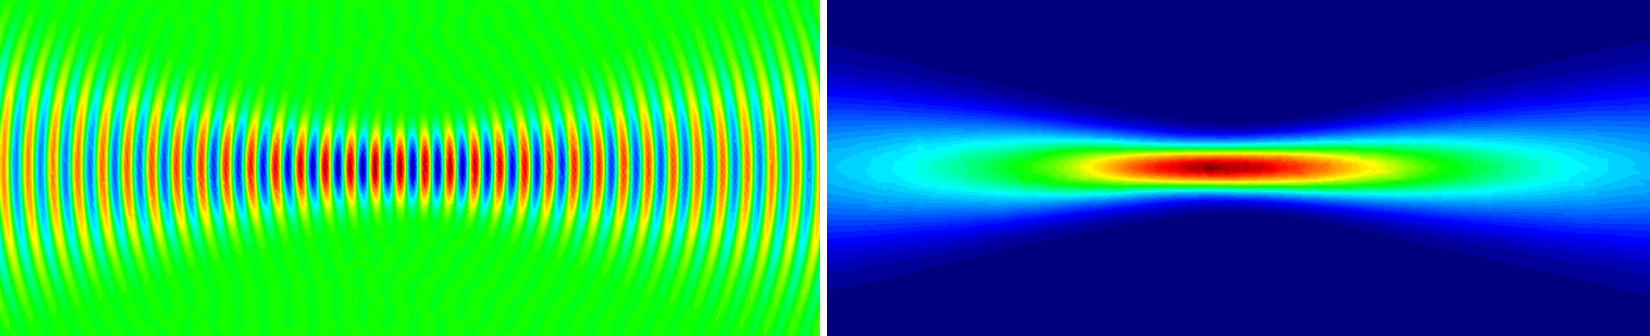
\includegraphics[width=\textwidth]{Contents/Figures/GaussBeamEzSx-W.png}
		\caption{Electric field (left) and Poynting vector (right) of a Gaussian beam in vacuum \cite{ERMES-O-X}.}
	\end{center}
\end{figure}

\begin{figure}[H]
	\begin{center}
		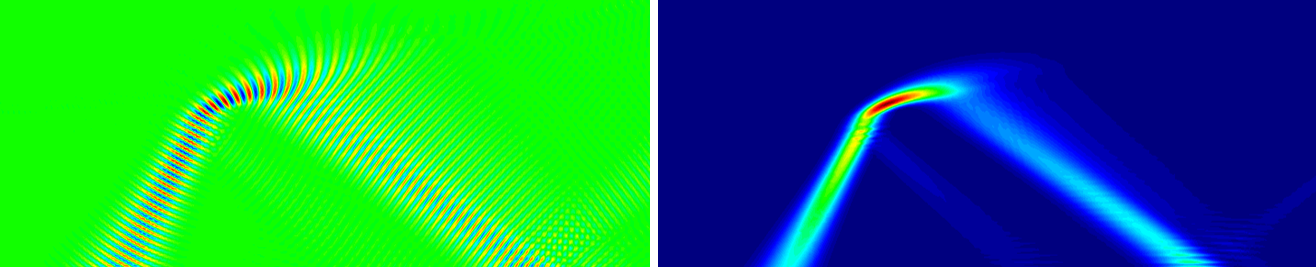
\includegraphics[width=\textwidth]{Contents/Figures/GaussBeamEzS-CP.png}
		\caption{Electric field (left) and Poynting vector (right) of a 20 GHz Gaussian beam in cold plasma \cite{ERMES-O-X}.}
	\end{center}
\end{figure}

\begin{figure}[H]
	\begin{center}
		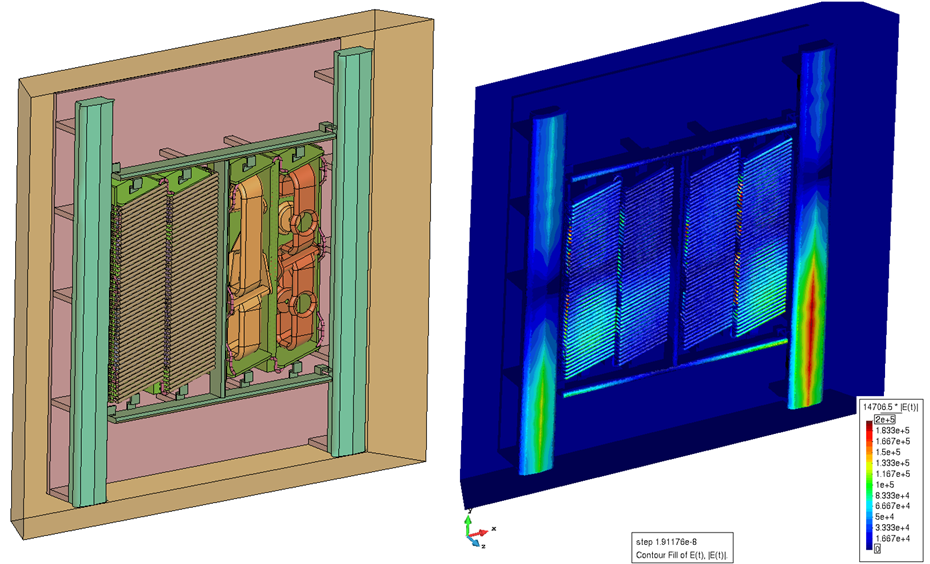
\includegraphics[width=\textwidth]{Contents/Figures/JET-A2-E-3D.png}
		\caption{Electric field generated by the JET A2 antenna in cold plasma \cite{ERMES-JET-A2}.}
	\end{center}
\end{figure}

\begin{figure}[H]
	\begin{center}
		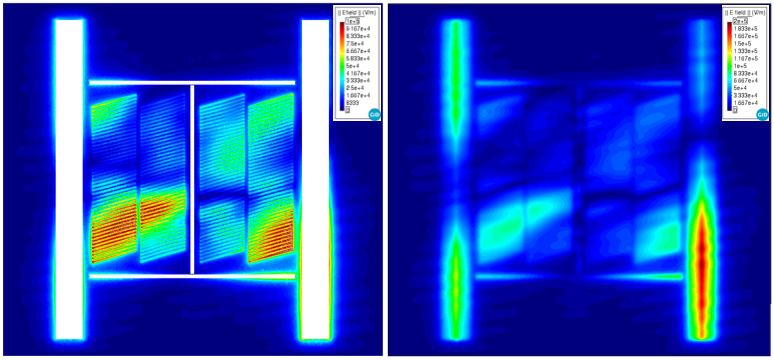
\includegraphics[width=\textwidth]{Contents/Figures/JET-A2-E-FRT.png}
		\caption{Cut planes of the electric field generated by the JET A2 antenna in cold plasma \cite{ERMES-JET-A2}.}
	\end{center}
\end{figure}

\begin{figure}[H]
	\begin{center}
		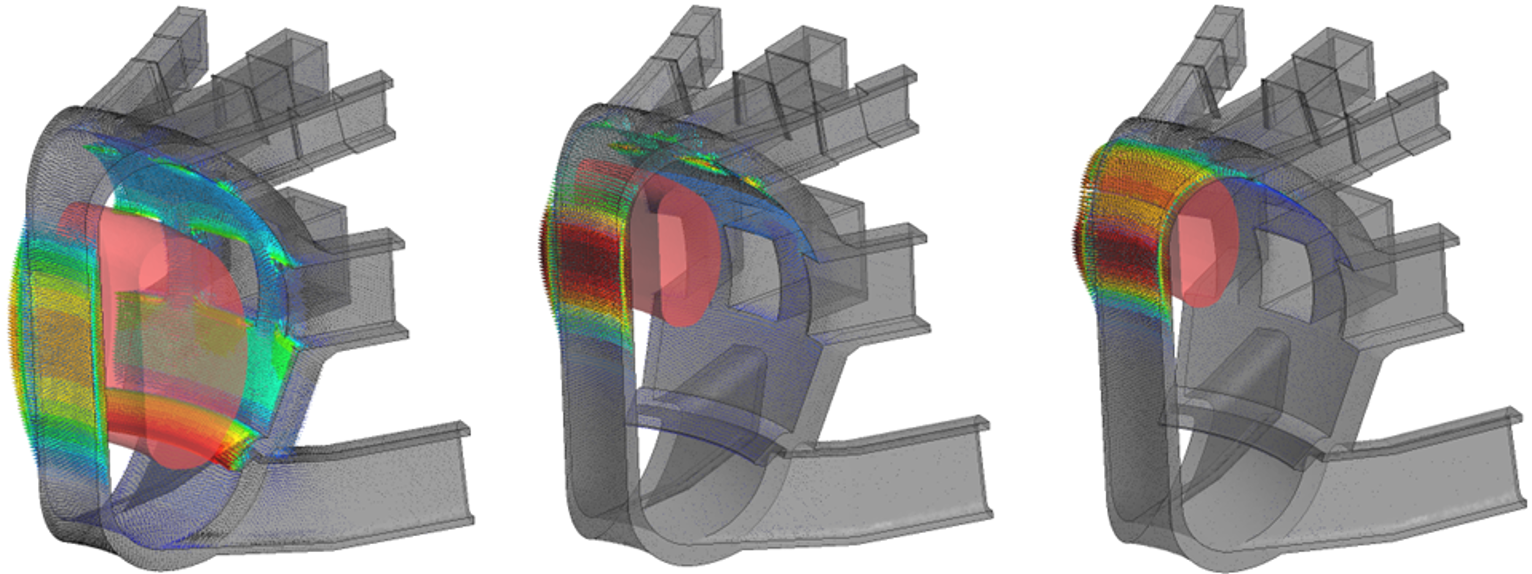
\includegraphics[width=\textwidth]{Contents/Figures/Disruption-ITER.png}
		\caption{Eddy currents induced on ITER walls by plasma disruption \cite{APS-DPP-2023}.}
	\end{center}
\end{figure}

\begin{figure}[H]
	\begin{center}
		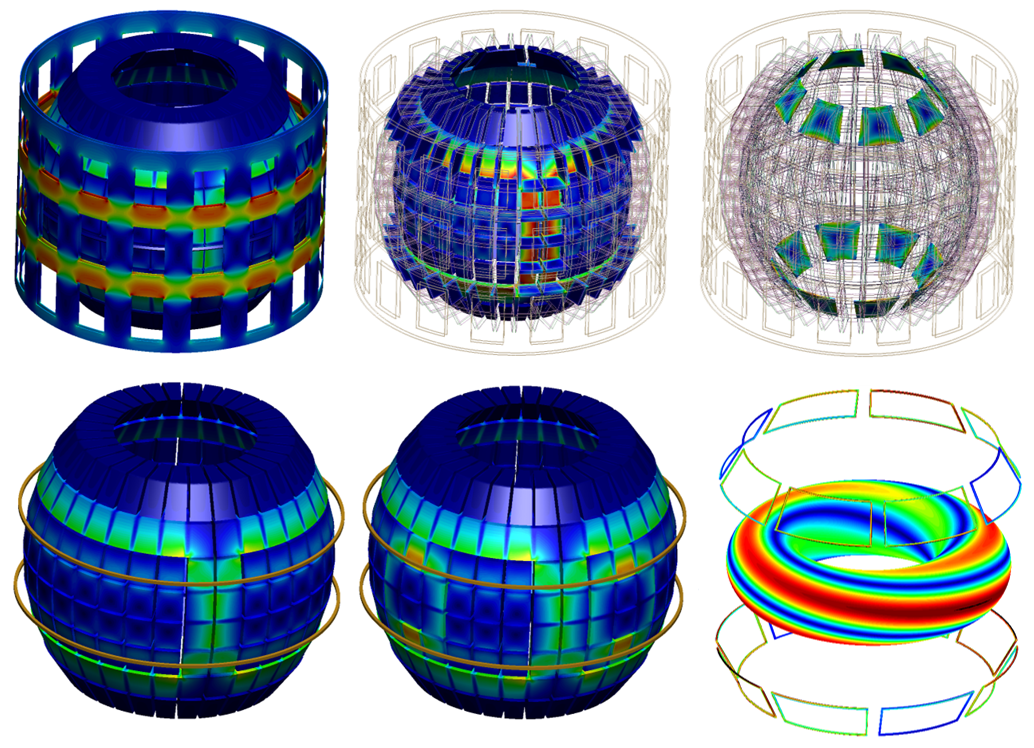
\includegraphics[width=\textwidth]{Contents/Figures/STEP-EddyCurrents.png}
		\caption{Eddy currents induced on STEP components by plasma and control coils \cite{APS-DPP-2023}.}
	\end{center}
\end{figure}

\begin{figure}[H]
	\begin{center}
		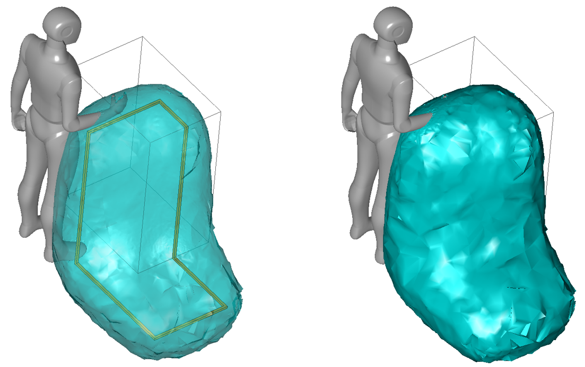
\includegraphics[width=\textwidth]{Contents/Figures/Dummy-IsoSurf.png}
		\caption{Iso-surfaces representing electromagnetic field exposure limits \cite{WedingEUDirective}.}
	\end{center}
\end{figure}

\begin{figure}[H]
	\begin{center}
		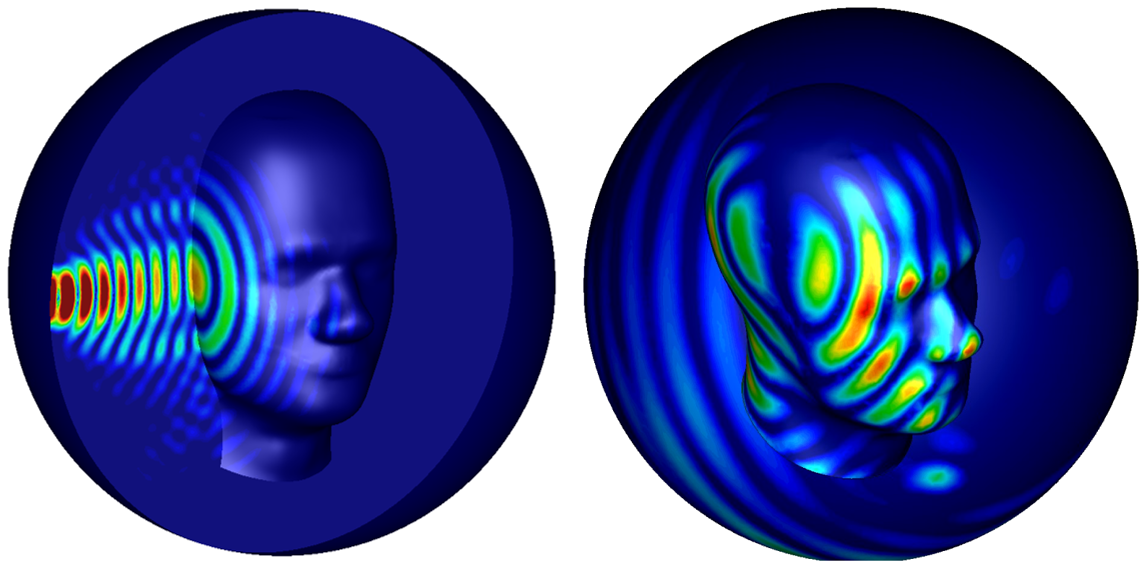
\includegraphics[width=\textwidth]{Contents/Figures/Head-Gaussian.png}
		\caption{Gaussian beams on SAM head.}
	\end{center}
\end{figure}

\begin{figure}[H]
	\begin{center}
		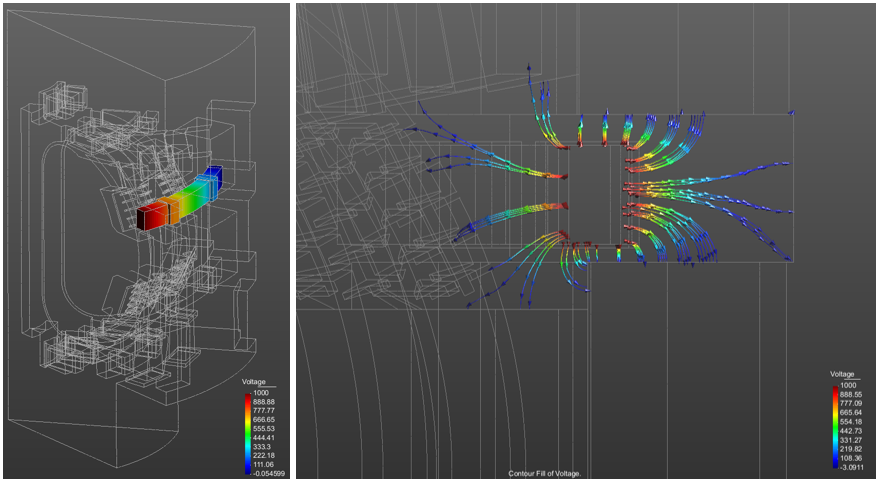
\includegraphics[width=\textwidth]{Contents/Figures/ITER-Quench-Voltage.png}
		\caption{Voltage induced by a quench in a superconducting poloidal coil of ITER.}
	\end{center}
\end{figure}

\begin{figure}[H]
	\begin{center}
		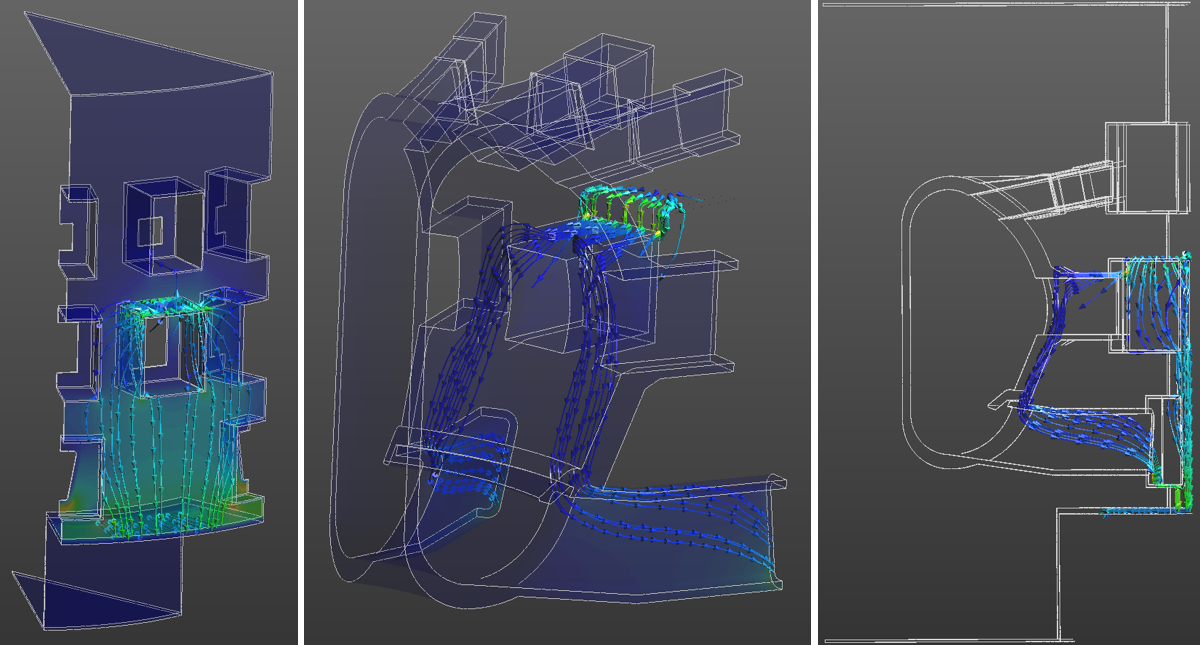
\includegraphics[width=\textwidth]{Contents/Figures/ITER-Arc-J.png}
		\caption{Electric currents following an electric arc strike on ITER components.}
	\end{center}
\end{figure}

\begin{figure}[H]
	\begin{center}
		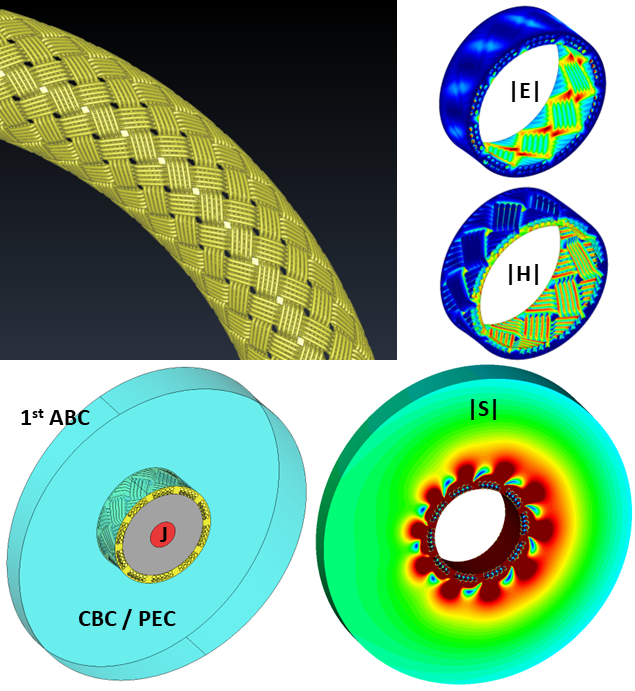
\includegraphics[width=\textwidth]{Contents/Figures/BWShield.png}
		\caption{Electromagnetic radiation leaking from a curved coaxial cable braided shield.}
	\end{center}
\end{figure}




